
\subsection{水治理变化的驱动力分析}
\label{Res.2}

\begin{figure*}[th!]
	\centering
	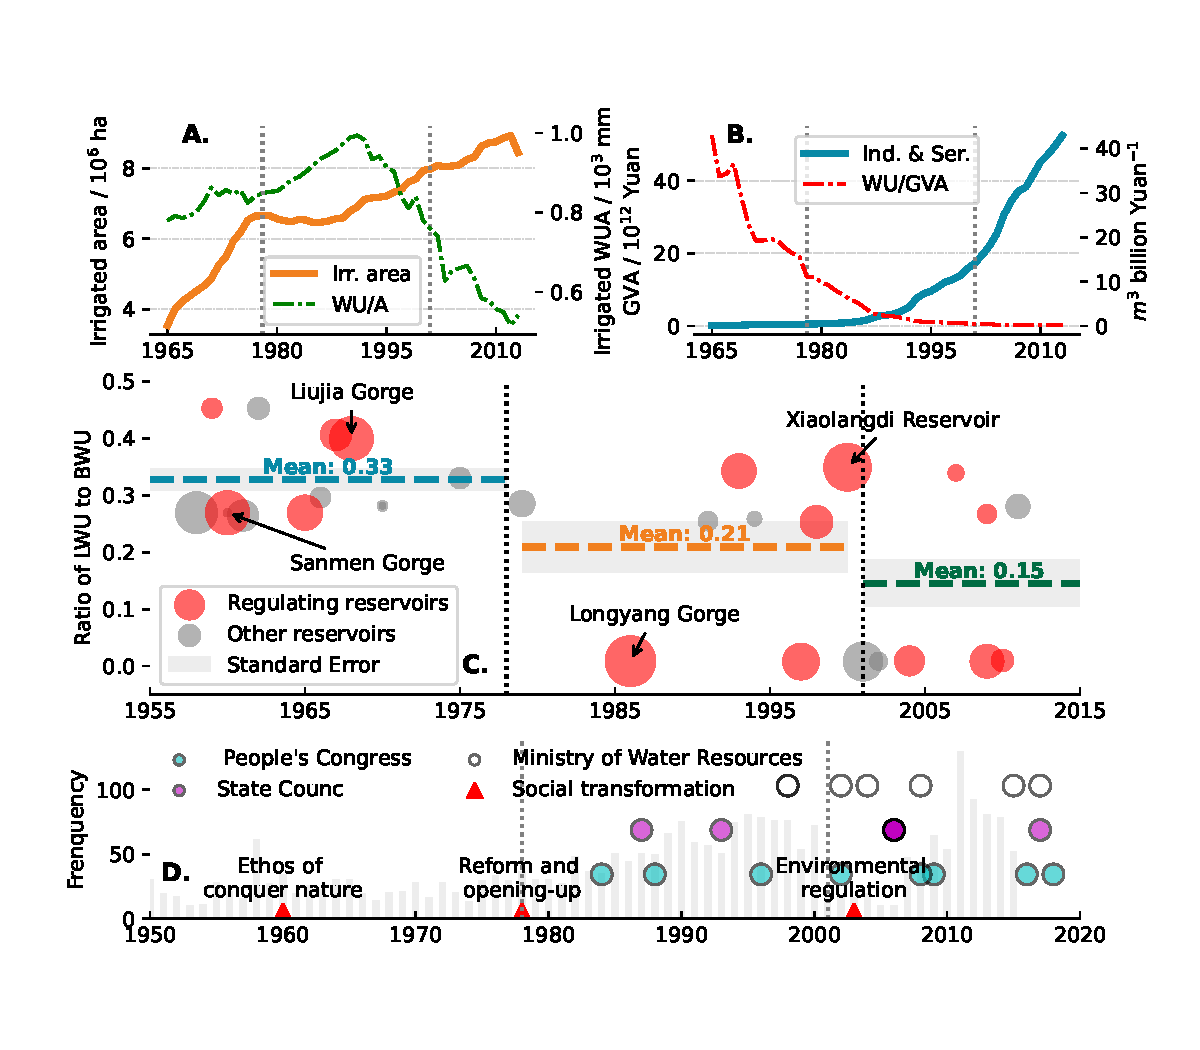
\includegraphics[width=0.9\linewidth]{img/ch4/causes.pdf}
	\caption{
		黄河流域水治理体制变化的原因。
		\textbf{A.}总灌溉面积(橙色线)和用水强度($WU/A$,用水量除以灌溉面积,绿点线)的变化。
        \textbf{B.}工业和服务业(蓝线)的总增加值(GVA)变化及其用水强度($WU/GVA$ WU除以GVA,红点线)。
        \textbf{C.}每个新水库的完工时间及其所在区域的用水量(LWU)占当时盆地总用水量(BWU)的百分比。红圈为主要管理和调节整个盆地的储层。每个圆圈的大小表示其储水能力的大小。
        \textbf{D.}社会转型(红色三角形)和国家层面的治理政策(圆圈,不同颜色表示由不同的国家机构签署,见表\ref{ch4:tab:policies})。浅灰色条形图以流域尺度(黄河事件)计算与黄河流域有关的官方文件。
	}
	\label{ch4:fig:mechanism}
\end{figure*}


\begin{figure}[tb]
    \centering
    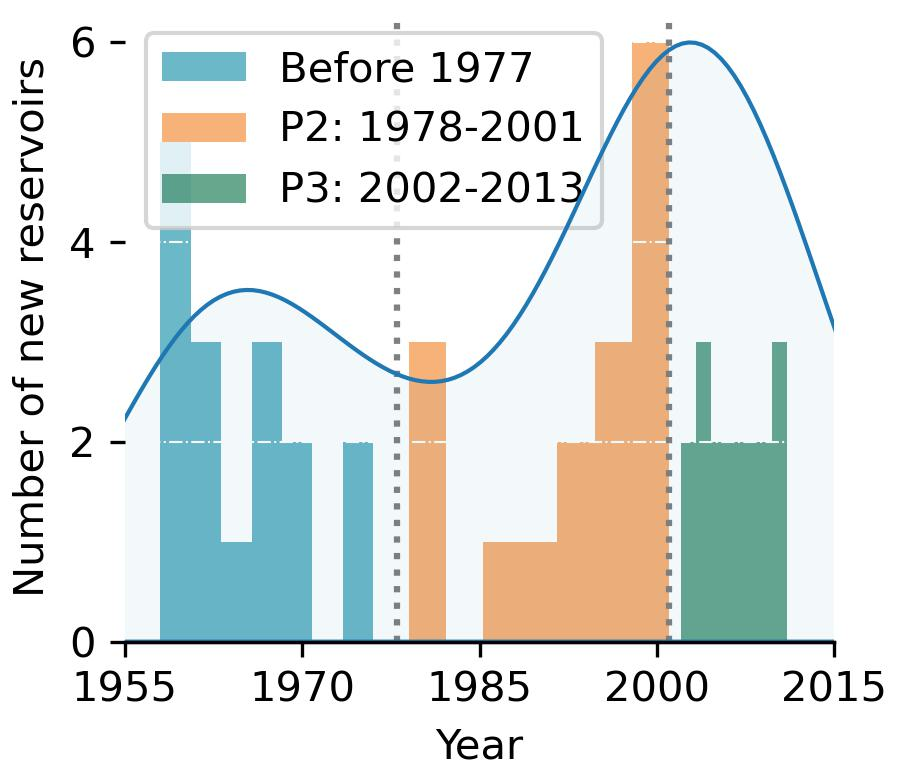
\includegraphics[width=0.6\linewidth]{img/ch4/reservoirs.jpg}
    \caption{
        各年新增水库数量.
    }
    \label{ch4:fig:reservoirs}
\end{figure}


进一步挖掘IWGI变化的根本原因。
灌溉区扩张和工业和服务业的经济增长是P1和P2目的变化的关键。
作为P1时期的主要用水需求,黄河流域的灌溉农业面积以100的速度迅速扩张(图\ref{ch4:fig:mechanism}~A),同时通过建设水库增加供应(图~\ref{ch4:fig:reservoirs})。
然而,进入P2后,灌溉区扩张停滞,工业和服务业逐渐增长,共同推动用水需求增加(图\ref{ch4:fig:mechanism}~A and B)。
接下来的P2到P3,水分利用效率变化最明显。
在P3期间,不仅灌溉区域继续缓慢扩张(图\ref{ch4:fig:mechanism}~A),而且工业和城市服务也承担了更重要的经济角色(由总增加值(GVA)表示)(图\ref{fig: Causes}~B)。
然而,由于效率的提高,单位灌溉面积或单位产量的用水量都显著下降(图~\ref{ch4:fig:mechanism}~A和图~\ref{ch4:fig:mechanism}~B)。
因此,在P3期间,部门和地区之间的用水差异减小,而总水压力稳定保持在较高水平(图~\ref{ch4:fig:IWGI}~A)。

最后,环境背景、社会转型和水治理政策在这三个时期的指标变化都发挥了作用。
我们计算了每个水库的区域用水量和流域用水量之比(区域/流域比值)(图~\ref{ch4:fig:mechanism}~C),因此较高的比值代表了在供水方面的潜在作用,而不是流域调度。
在P1时期“征服自然”的旗帜下,大部分水库都建在需水量较大的地区,因此R/B比值明显较高($p<0.01$,见图~\ref{ch4:fig:mechanism}~C)。
进入P2期之后,新水库数量明显减少,流域政策严格控制了水的分配(图~\ref{ch4:fig:mechanism}~D, $p<0.01$和图\ref{ch4:fig:reservoirs})。
在P3阶段,当局在“环境规制”国家战略的指导下提出了更多的、级别更高的水治理政策(图~\ref{ch4:fig:mechanism}~D)。
从P1到P2的状态转变与水资源供需的增加相一致,而在P2到P3稳定的水压力下,则是由监管政策和效率提高所驱动的。